\section{Doménový model}
V předchozí podkapitole byla představena MVC architektura a byly popsány její vrstvy. Tato podkapitola se zaměřuje na vrstvu modelů a bude v ní podrobněji představeno s jakými daty bude nová aplikace pracovat. Ke znázornění modelů, jejich vlastností a vazeb mezi nimi je využit doménový model, který je na obrázku \ref{figure:domain-model}. Doménový model obsahuje u každé třídy (entity) všechny vlastnosti, které se u ní plánují evidovat. Povinné vlastnosti entit jsou označeny symbolem $ \star $.

\begin{landscape}
	\begin{figure}[h]
		\caption{Doménový model}
		\label{figure:domain-model}
		\centering
		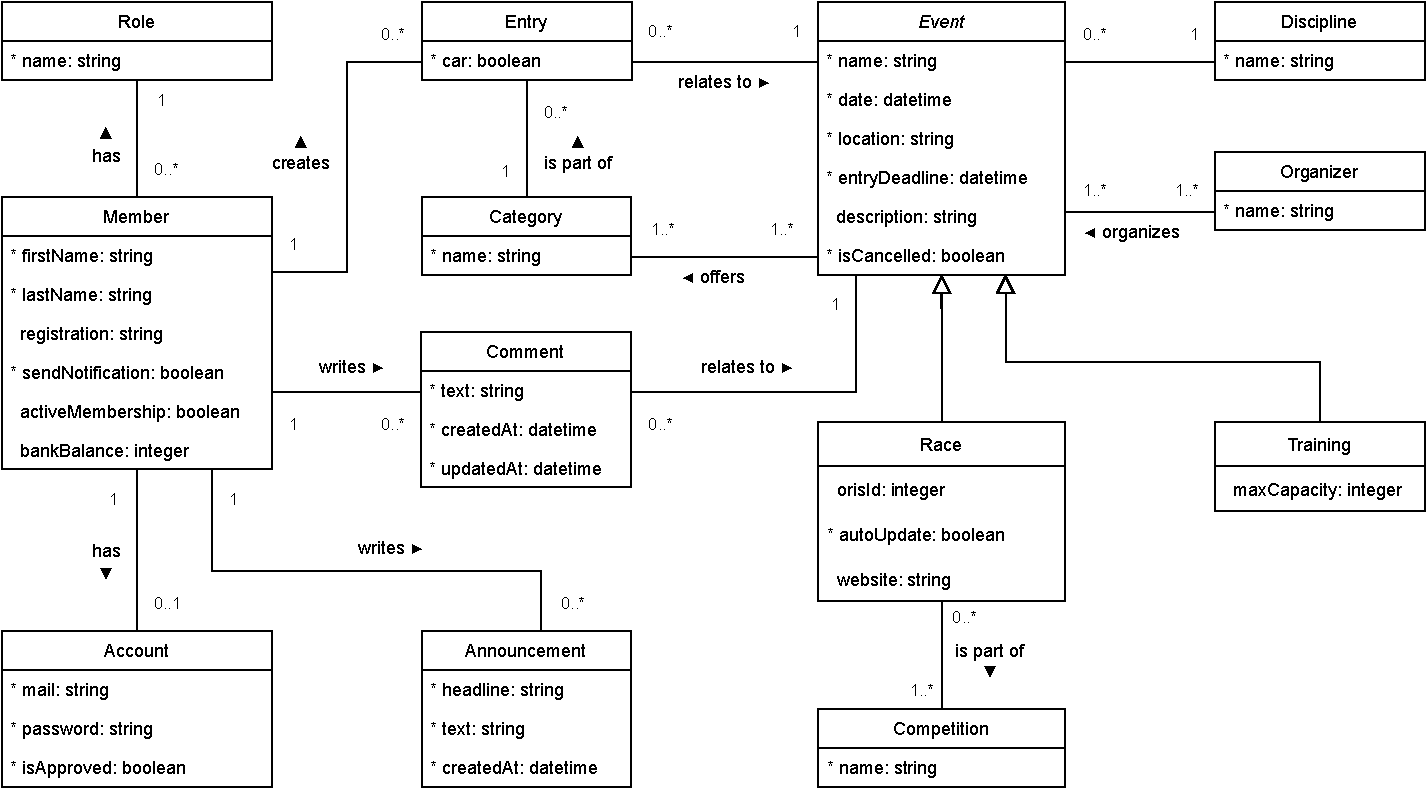
\includegraphics[width=0.96\linewidth]{images/domain-model.pdf}
	\end{figure}
\end{landscape}
